% Drawing 154/06-21 -- folder 154, batch 06, archive page 104 (PDF page 105).
% Transcription: une rangée de cinq dessins en couleur reliés par des flèches $\mapsto$ : un cycle de positions relatives d'une droite vert clair par rapport à deux paires de droites orange et à un faisceau de droites parallèles ; la droite verte contourne tour à tour l'un ou l'autre croisement, l'arc $a$ et, en pointillé, l'arc $b$ sont marqués, et des flèches $\leftarrow$, $\rightarrow$ donnent l'orientation. Les dessins sont étiquetés $(1)$, $(2)$, $(3)$, $(4)$, $(1)$, le dernier revenant au premier ; les secteurs hachurés au crayon portent des numéros entourés
% Kind: cycle of five relative positions. Method 2 (schematic redraw from the facsimile). Status: partial.
% Notes: Five positions joined by four arrows. (1): the line under both crossings, the arc a black at the first, b dotted at the second, four parallel strokes between them, arrow to the left. (2): the line makes a bump over the first crossing, a black stroke on top of it, the black arc at the second, arrow to the right. (3): two bumps, over both crossings, arrow to the left. (4): the line (dark green on the left) passes under the first crossing, dotted arc there, and over the second, arrow to the right. (1) again. Crossings computed. Left out: the pencil hatching of the sectors, most of the circled numbers (those drawn are 1, 4', 2, 1', 3, 2', 3'; one near the top of the last drawing reads « 5 = 1 » and is not drawn), the Greek letters on the parallel strokes other than lambda, lambda' in the first drawing, and two struck marks under the labels (1) and (3). Redrawn 2026-11-12 (issue 128): to check again. 2026-11-14, Claude Opus 5.5, overlay check (issue 147): rasterised from its own coordinates over the 400 dpi colour scan (402 ppi native) on a unit grid; not compiled (no TeX in the session). The five positions: the orange crossings, the light green line with its bumps, the black and dotted arcs, the parallel strokes, the arrows and the labels (1) to (4) lie on their ink to within about 1 to 1.5 units; the redraw is unchanged. Still differs, hence partial: the pencil hatching of the sectors, which the transcription names, is not drawn, nor are most of their circled numbers, the Greek letters of the parallel strokes and the circled « 5 = 1 » above the last drawing.
% Coordinates: 1 unit = 1 mm = 1/100 of the crop width (bbox in page fractions: [0.14, 0.125, 0.93, 0.215]).
% Redrawn by Claude (claude-fable-5-2), issue #128, 2026-11-12; not checked by a human; not compiled (no TeX in the session).
% Checked by Claude (claude-opus-5-5) 2026-11-14 (issue #147): overlaid on the 400 dpi colour facsimile; not compiled (no TeX in the session). Not checked by a human. Status: partial.
% Rights: reproduces part of the work -- behind RENDER_TRANSCRIPTS, never published by itself.
\documentclass[tikz,border=3pt]{standalone}
\usepackage{amsmath,amssymb}
\usetikzlibrary{patterns,arrows.meta}
\tikzset{Or/.style={orange!90!black}, Lg/.style={green!60!black!70}, Dg/.style={green!45!black}, pencil/.style={black!45}, struck/.style={black!35}, mpt/.style={circle,draw,inner sep=1.3pt}, pt/.style={circle,fill,inner sep=0.9pt}, opt/.style={circle,draw,fill=white,inner sep=1.1pt}}
\begin{document}
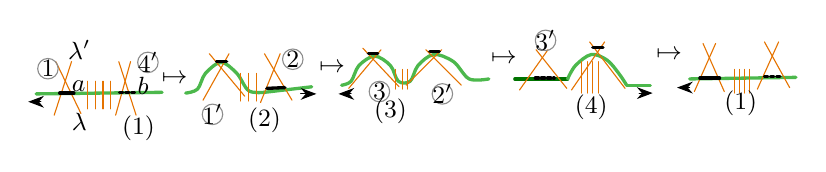
\begin{tikzpicture}[x=1mm,y=1mm,line cap=round,line join=round,font=\scriptsize]
\draw[Lg,very thick] (2,-9.6) -- (18,-9.4);
\draw[Or] (4.5,-5.5) -- (7.7,-12.1);
\draw[Or] (6.5,-5.5) -- (4.3,-12.3);
\draw[very thick] (5,-9.5) -- (6.8,-9.5);
\node[inner sep=1pt] at (7.4,-8.6) {\small $a$};
\draw[Or] (8.5,-8) -- (8.5,-11.5);
\draw[Or] (9.5,-8) -- (9.5,-11.5);
\draw[Or] (10.5,-8) -- (10.5,-11.5);
\draw[Or] (11.5,-8) -- (11.5,-11.5);
\draw[Or] (12.5,-5.5) -- (14.7,-12.3);
\draw[Or] (14,-5.5) -- (12.1,-12.3);
\draw[densely dotted,very thick] (12.6,-9.4) -- (14.5,-9.4);
\node[inner sep=1pt] at (15.6,-8.6) {\small $b$};
\draw[-{Stealth[length=2mm]}] (2.6,-10.6) -- (1,-10.6);
\draw[pencil] (3.5,-6.4) circle[radius=1.3];
\node[inner sep=1pt] at (3.5,-6.4) {\small 1};
\draw[pencil] (16.2,-5.6) circle[radius=1.3];
\node[inner sep=1pt] at (16.2,-5.6) {\small $4'$};
\node[inner sep=1pt] at (15,-14) {\small (1)};
\node[inner sep=1pt] at (19.6,-7.7) {\small $\mapsto$};
\draw[Lg,very thick] plot[smooth, tension=0.55] coordinates {(21,-9.5) (22.5,-9) (23.5,-7) (25.5,-5.6) (27.5,-7) (29,-9.2) (31,-9.4)};
\draw[Lg,very thick] (31,-9.4) -- (37,-8.7);
\draw[Or] (24,-4.5) -- (28.5,-9.9);
\draw[Or] (26.5,-4.5) -- (23.2,-10.4);
\draw[very thick] (24.9,-5.5) -- (26.2,-5.5);
\draw[Or] (28,-7) -- (28,-10.5);
\draw[Or] (29,-7) -- (29,-10.5);
\draw[Or] (30,-7) -- (30,-10.5);
\draw[Or] (31,-4.5) -- (34.5,-10.4);
\draw[Or] (33,-4.5) -- (30.5,-10.7);
\draw[very thick] (31.3,-8.9) -- (33.6,-8.8);
\draw[-{Stealth[length=2mm]}] (35.6,-9.6) -- (37.6,-9.6);
\draw[pencil] (34.6,-5.2) circle[radius=1.3];
\node[inner sep=1pt] at (34.6,-5.2) {\small 2};
\draw[pencil] (24.4,-12.2) circle[radius=1.3];
\node[inner sep=1pt] at (24.4,-12.2) {\small $1'$};
\node[inner sep=1pt] at (31,-13) {\small (2)};
\node[inner sep=1pt] at (39.6,-6.3) {\small $\mapsto$};
\draw[Lg,very thick] plot[smooth, tension=0.55] coordinates {(40.8,-8.5) (42,-8) (43,-6) (45,-4.8) (47,-6) (48,-8) (49.5,-8) (50.5,-6) (52.5,-4.6) (55,-5.5) (57,-7.7) (59.5,-7.7)};
\draw[Or] (43.5,-3.8) -- (48.1,-8.7);
\draw[Or] (45.8,-4) -- (41.7,-8.9);
\draw[Or] (51.5,-4) -- (56,-8.5);
\draw[Or] (53.5,-4) -- (49,-8.5);
\draw[very thick] (44.2,-4.5) -- (45.4,-4.5);
\draw[very thick] (52,-4.2) -- (53.2,-4.2);
\draw[Or] (47.7,-6.5) -- (47.7,-9);
\draw[Or] (48.5,-6.5) -- (48.5,-9);
\draw[Or] (49.2,-6.5) -- (49.2,-9);
\draw[-{Stealth[length=2mm]}] (42,-9.6) -- (40.4,-9.6);
\draw[pencil] (45.6,-9.3) circle[radius=1.3];
\node[inner sep=1pt] at (45.6,-9.3) {\small 3};
\draw[pencil] (53.6,-9.6) circle[radius=1.3];
\node[inner sep=1pt] at (53.6,-9.6) {\small $2'$};
\node[inner sep=1pt] at (47,-11.8) {\small (3)};
\node[inner sep=1pt] at (61.4,-5.2) {\small $\mapsto$};
\draw[Dg,very thick] (62.8,-7.7) -- (69.5,-7.7);
\draw[Lg,very thick] plot[smooth, tension=0.55] coordinates {(69.5,-7.7) (70.5,-6) (72.5,-4.6) (74.5,-5.3) (76,-7) (77,-8.5)};
\draw[Lg,very thick] (77,-8.5) -- (80,-8.5);
\draw[Or] (65.5,-4) -- (69.4,-8.9);
\draw[Or] (67,-4) -- (63.4,-9.1);
\draw[densely dotted,very thick] (65.4,-7.6) -- (67.8,-7.6);
\draw[Or] (71.3,-5.5) -- (71.3,-9.5);
\draw[Or] (72,-5.5) -- (72,-9.5);
\draw[Or] (72.7,-5.5) -- (72.7,-9.5);
\draw[Or] (73.4,-5.5) -- (73.4,-9.5);
\draw[Or] (72.3,-3) -- (76.8,-8.9);
\draw[Or] (74.2,-3) -- (70,-9.1);
\draw[very thick] (72.7,-3.7) -- (74,-3.7);
\draw[-{Stealth[length=2mm]}] (78.6,-9.5) -- (80.3,-9.5);
\draw[pencil] (66.7,-2.8) circle[radius=1.3];
\node[inner sep=1pt] at (66.7,-2.8) {\small $3'$};
\node[inner sep=1pt] at (72.5,-11.3) {\small (4)};
\node[inner sep=1pt] at (82.4,-4.7) {\small $\mapsto$};
\draw[Lg,very thick] (85,-7.7) -- (98.5,-7.5);
\draw[Or] (86.7,-3.2) -- (89.4,-9.3);
\draw[Or] (88.3,-3.2) -- (85.6,-9.3);
\draw[very thick] (86.3,-7.6) -- (88.8,-7.6);
\draw[Or] (90.7,-6.5) -- (90.7,-9.5);
\draw[Or] (91.3,-6.5) -- (91.3,-9.5);
\draw[Or] (92,-6.5) -- (92,-9.5);
\draw[Or] (92.6,-6.5) -- (92.6,-9.5);
\draw[Or] (94.5,-3) -- (97.7,-8.8);
\draw[Or] (96.3,-3) -- (93.6,-9);
\draw[densely dotted,very thick] (94.5,-7.4) -- (96.5,-7.4);
\draw[-{Stealth[length=2mm]}] (85,-8.8) -- (83.4,-8.8);
\node[inner sep=1pt] at (91.5,-10.8) {\small (1)};
\node[inner sep=1pt] at (7.5,-4) {\small $\lambda'$};
\node[inner sep=1pt] at (7.5,-13.2) {\small $\lambda$};
\end{tikzpicture}
\end{document}
